\section{Application Implementations}
\label{appendix:appl-impl}

\begin{figure}
  \centering
  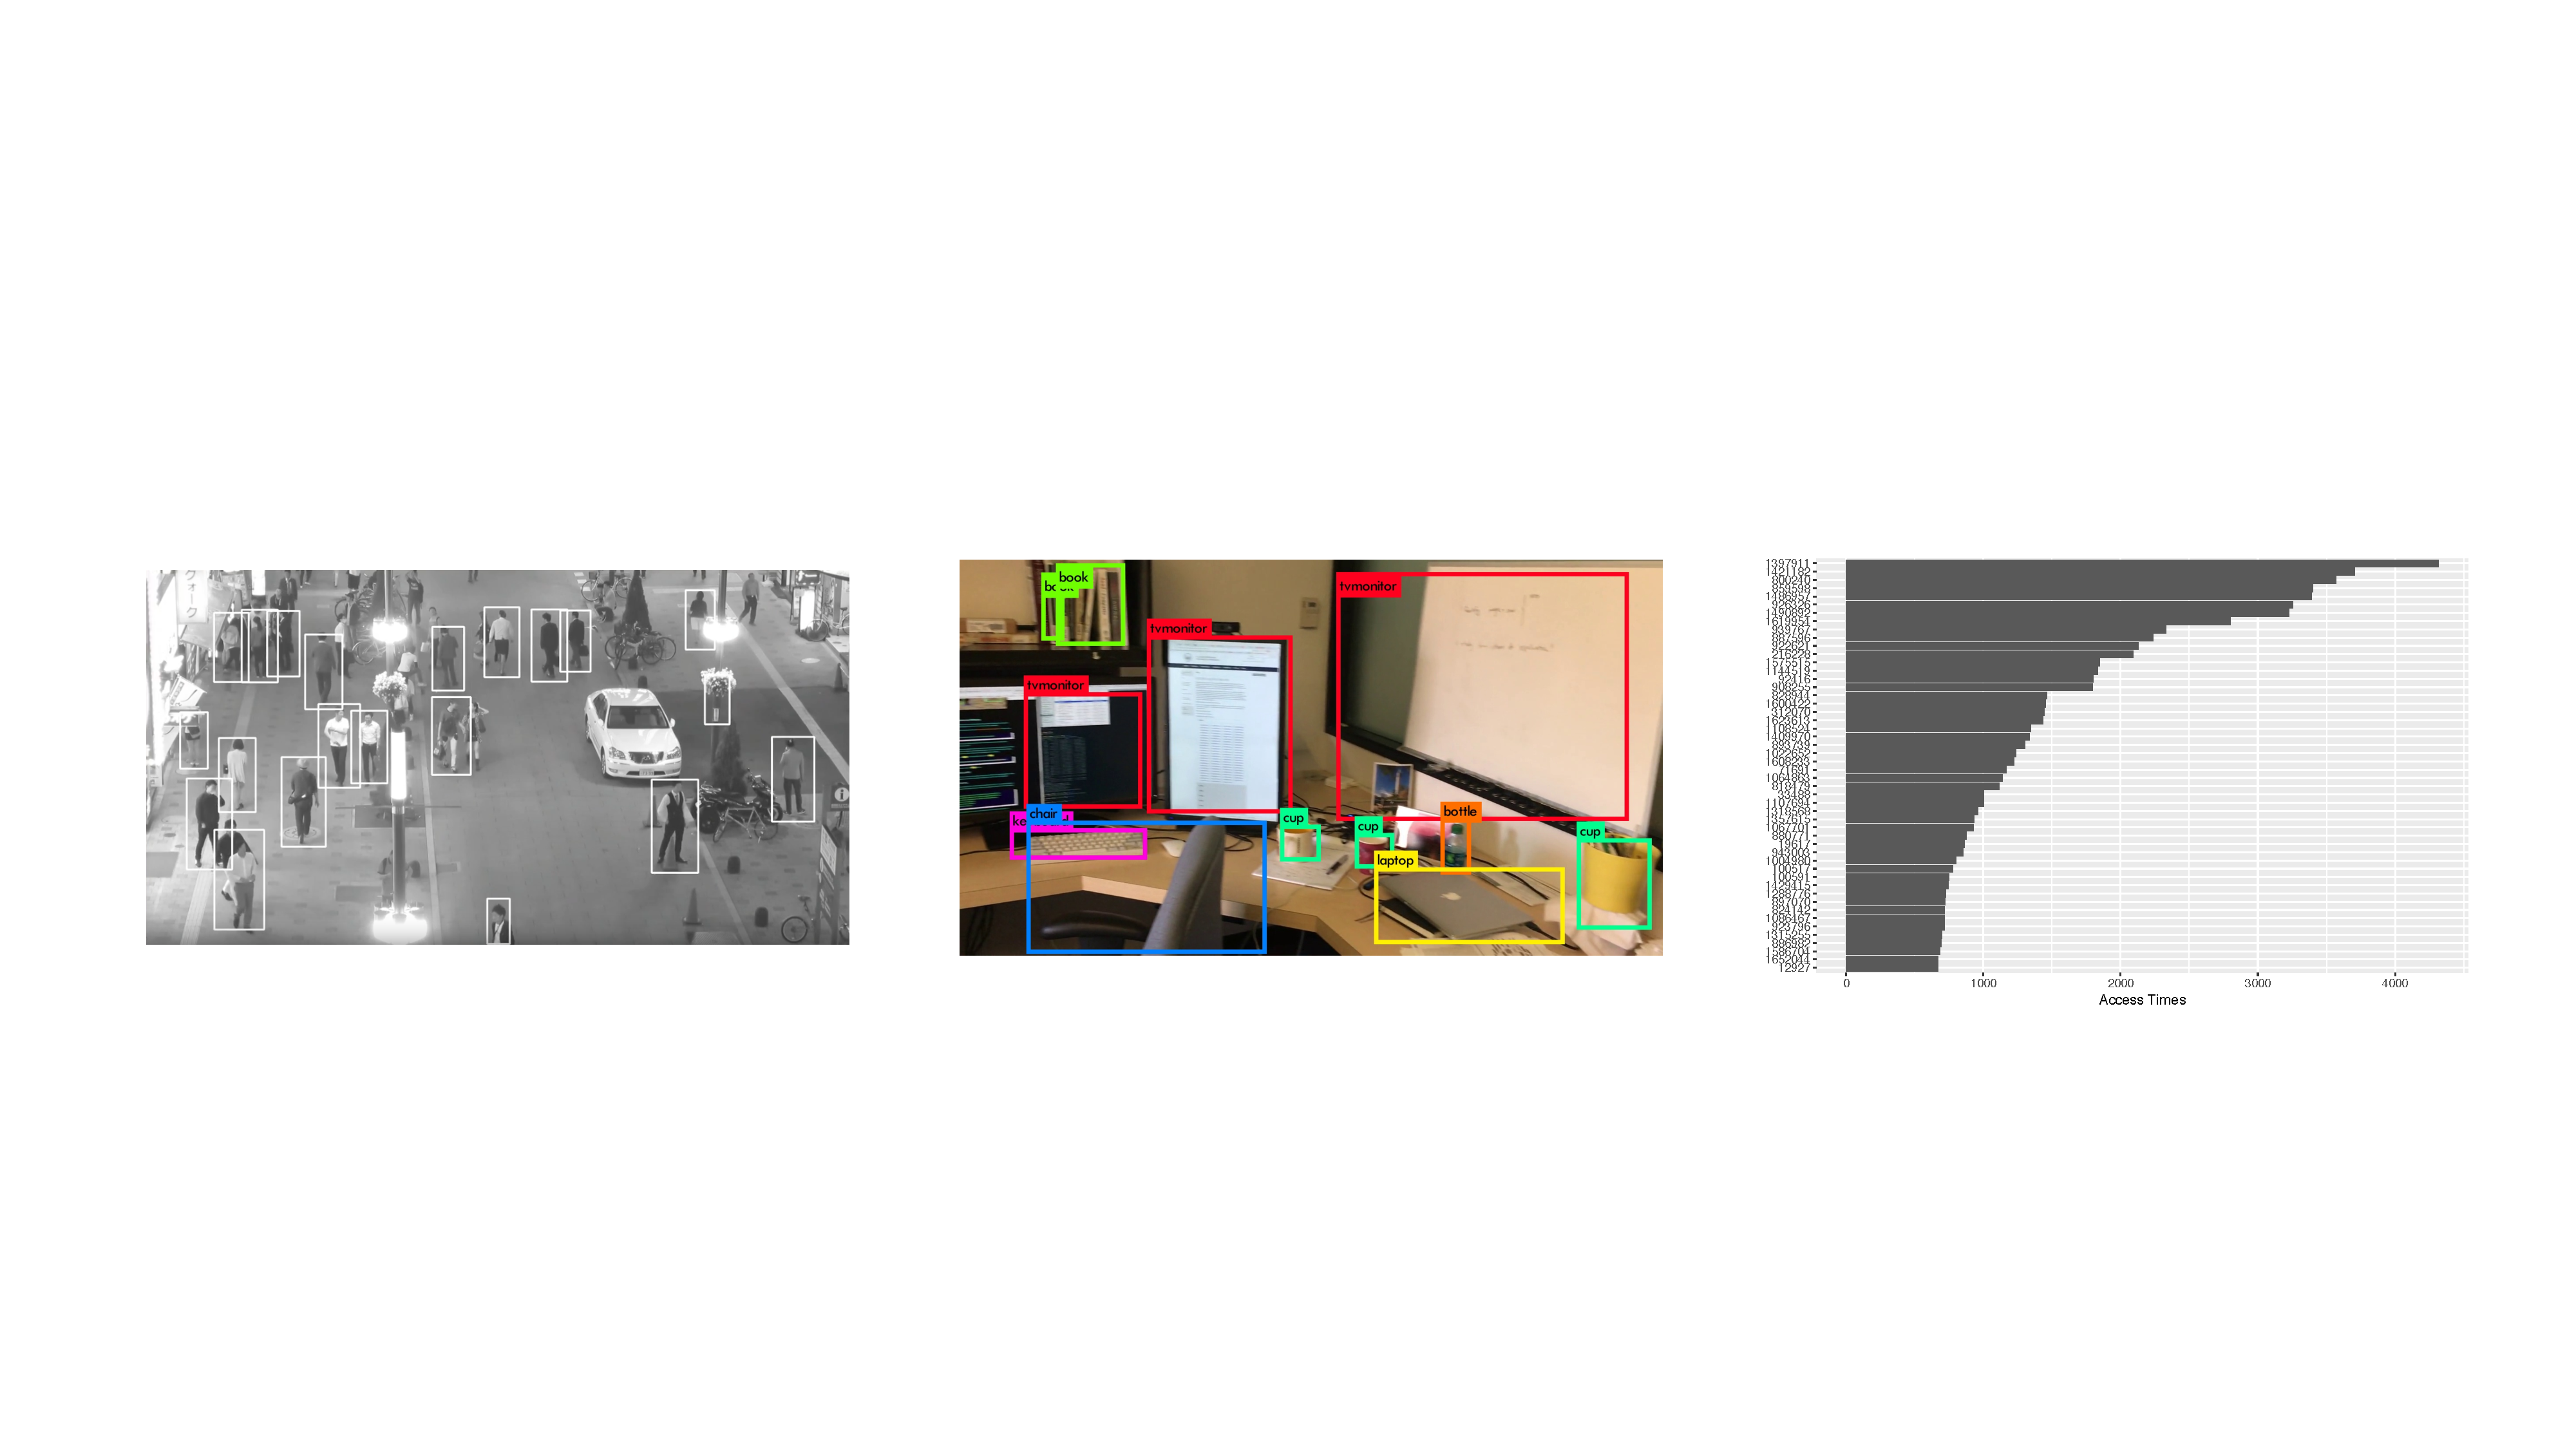
\includegraphics[width=\columnwidth]{figures/apps.pdf}
  \caption{Illustration of our three applications: pedestrian detection,
    augmented reality, and distributed Top-K.}
  \label{fig:three-apps}
\end{figure}

Below we provide details about how we implement our three applications
(\autoref{fig:three-apps}), including the libraries we use and how we integrate
them into \sysname{}.

\para{Augmented Reality.} We target mobile augmented reality applications that
recognizes objects by offloading the heavy computation to resources elsewhere.
We implement image-related operations with OpenCV 3.1~\cite{opencvlibrary} and
recognize objects using YOLO~\cite{darknet13, redmon2016yolo9000}, a GPU-enabled
pre-trained neural network. Video encoding employs H.264 because of its
prevalence in existing systems. Our implementation uses
GStreamer~\cite{gstreamer} with \texttt{x264enc} plugin. To integrate with
\sysname{}, we first create a pipeline that exposes \texttt{appsrc} (to feed raw
image data) and \texttt{appsink} (to get encoded bytes). The GStreamer main loop
executes in a separate thread and \sysname{} communicates with it via Rust's
channel. The \texttt{x264enc} uses the \texttt{zerolatency} preset and four
threads. We use constant quality encoding and expose the quantization factor as
another knob (in addition to image resolution and frame rate).

Object recognition returns a list of bounding boxes with the type of the object,
and each box is a rectangle with normalized coordinates on the image. We compare
the detection against the reference result from raw data, and declare it success
if the intersection over union (IOU) is greater than
50\%~\cite{everingham2010pascal} and the object type matches. We use F1
score~\cite{Rijsbergen:1979:IR:539927} as the accuracy function. In terms of
dataset, we've collected our own video clips: the training data is a 24-second
long video of an office environment; the test data is a 246-second long video of
a home environment.

\para{Pedestrian Detection.} This application analyzes streams of videos from
installed CCTV cameras and detects pedestrians inside. We use a similar setup
(OpenCV and GStreamer) as our augmented reality application except for the
analytical function. To detect pedestrians, we use histogram of oriented
gradients (HOG)~\cite{dalal2005histograms} with the default linear SVM
classifier. To ensure real-time processing of frames, we use the GPU-accelerated
implementation. Because we do not recognize individual pedestrians, a successful
detection in this case only requires matching the bounding box.  MOT16
dataset~\cite{milan2016mot16} is used for both training and testing.

\begin{figure}
  \centering
  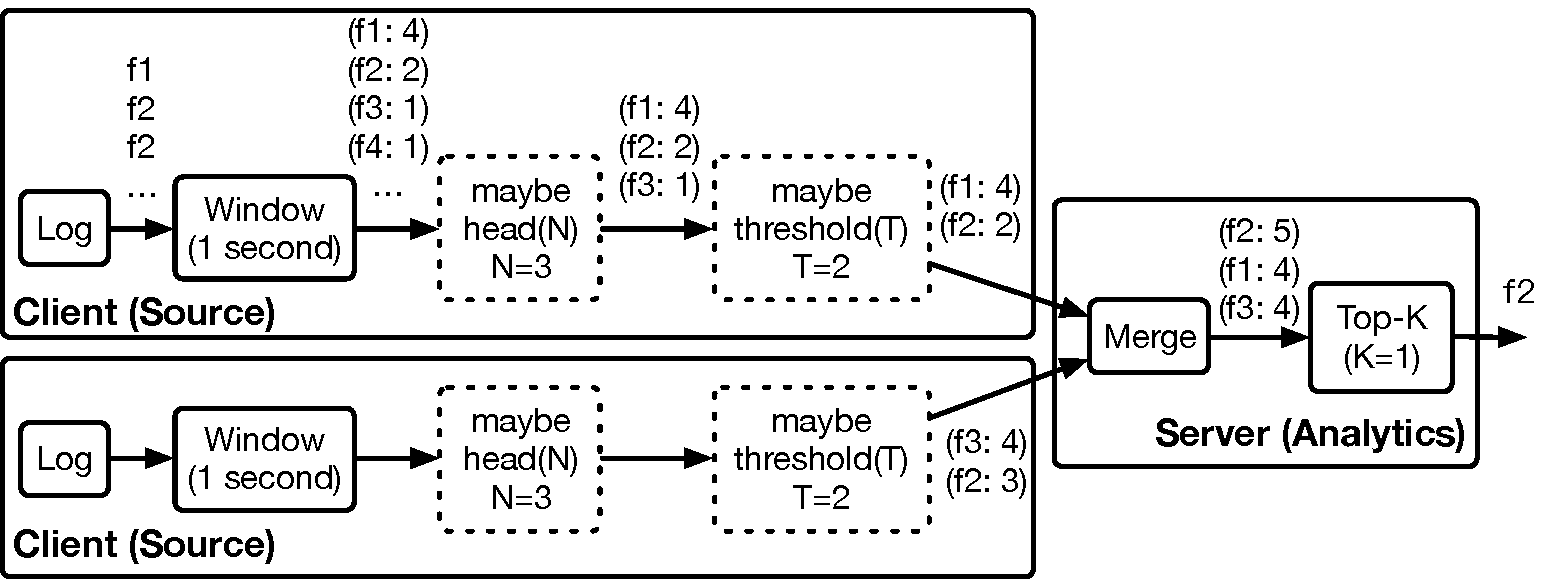
\includegraphics[width=\columnwidth]{figures/topk.pdf}
  \caption{A distributed Top-K application with two degradation operations:
    \texttt{head} and \texttt{threshold}.}
  \label{fig:topk}
\end{figure}


\para{Distributed Top-K.} Many monitoring applications need to answer the
\textit{Top-K} question~\cite{babcock2003distributed}, such as the Top-K most
popular URLs, or the Top-K most access files. A distributed Top-K application
aggregates information from geo-distributed servers to computer a final Top-K.

\autoref{fig:topk} shows the Top-K processing pipeline. Edge nodes can first
perform a \texttt{Window} operation to generate data summary, such as key-value
pairs of \texttt{<item, count>}. After the summary, the data size can still be
too large because most real-world access patterns follow a long tail
distribution. There is a large-but-irrelevant tail that contributes little to
Top-K. The edge nodes perform two degradation operations: (1) a head
(\texttt{N}) operation that only takes the top \texttt{N} entries; (2) a
threshold \texttt{T} that filters small entries. These two operations are not
orthogonal. Their impact on data size reduction and quality degradation depends
on the data distribution.

For accuracy, we use Kendall's~$\tau$~\cite{abdi2007kendall}, a correlation
measure of the concordance between two ranked list. The output ranges from
\(-1\) to 1, representing no agreement to complete agreement. To integrate with
\sysname{}, we convert Kendall's~$\tau$ to the range of [0, 1] with a linear
transformation.

Our Top-K application aims to find the Top-50 most accessed files from web
server logs. We use Apache log files that record and store user access
statistics for the \href{https://www.sec.gov}{SEC.gov} website. The logs are
split into four groups, simulating four geo-distributed nodes monitoring web
accesses. To match the load of popular web servers, we compress one hour's logs
into one second.

\section{Runtime Experiments}
\label{appendix:more-runtime}

\begin{figure}[t]
  \begin{subfigure}[t]{\columnwidth}
    \centering
    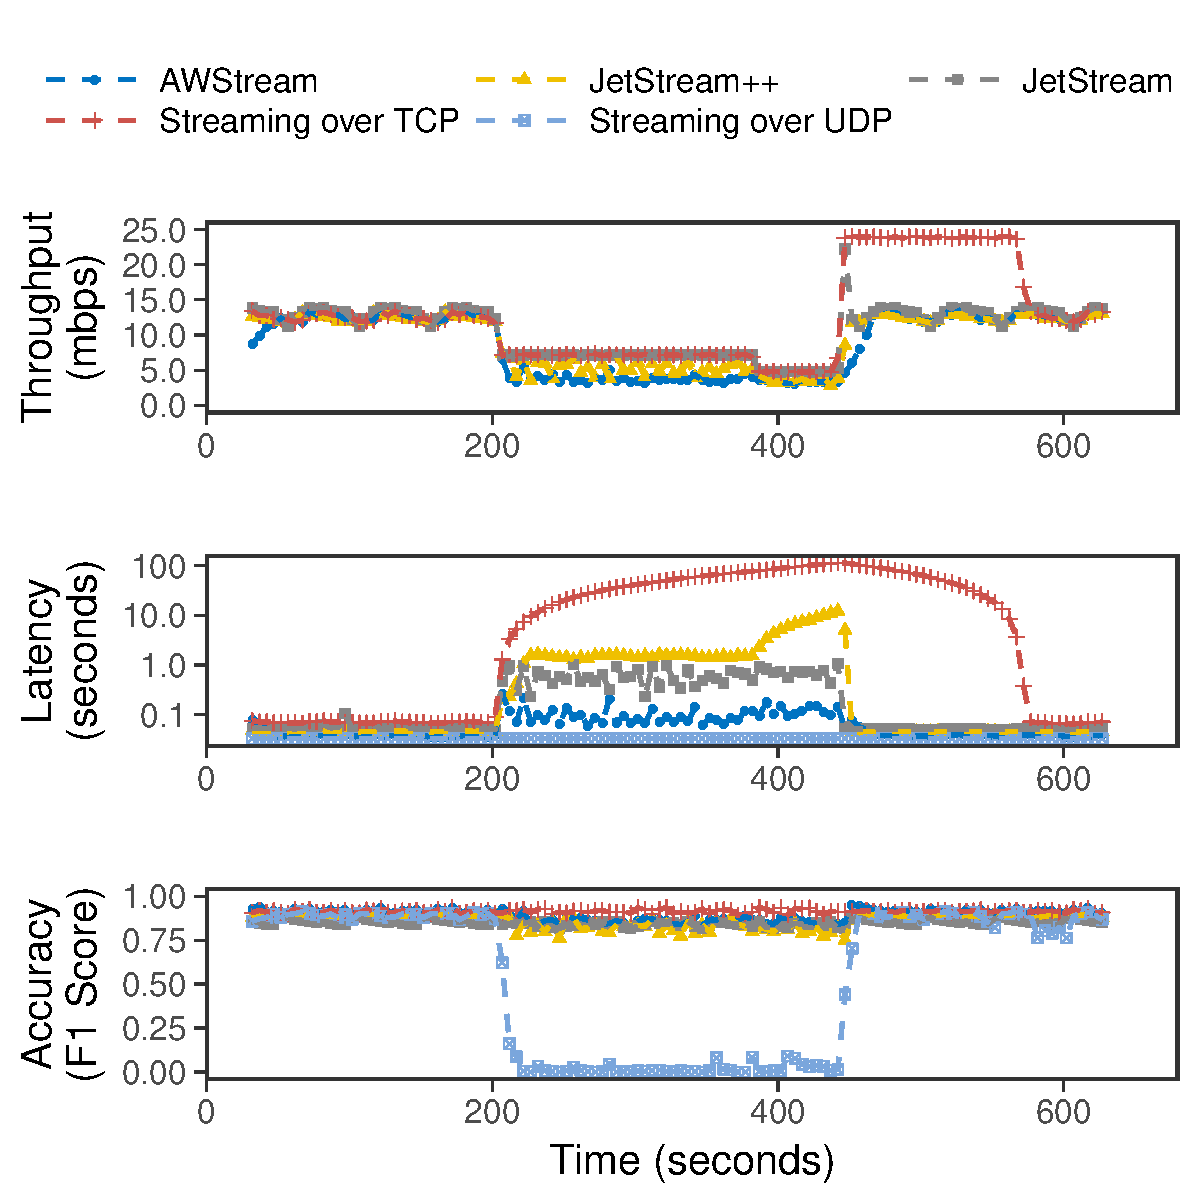
\includegraphics[width=\columnwidth]{figures/runtime_mot-timeseries.pdf}
    \caption{PD's runtime behavior with a time-series plot: throughput (top),
      showing the effect of bandwidth shaping; latency (middle) in log scale;
      and accuracy (bottom).}
    \label{fig:pd-runtime-timeseries}
  \end{subfigure}
  \vspace{1em}
  \\
  \begin{subfigure}[t]{\columnwidth}
    \centering
    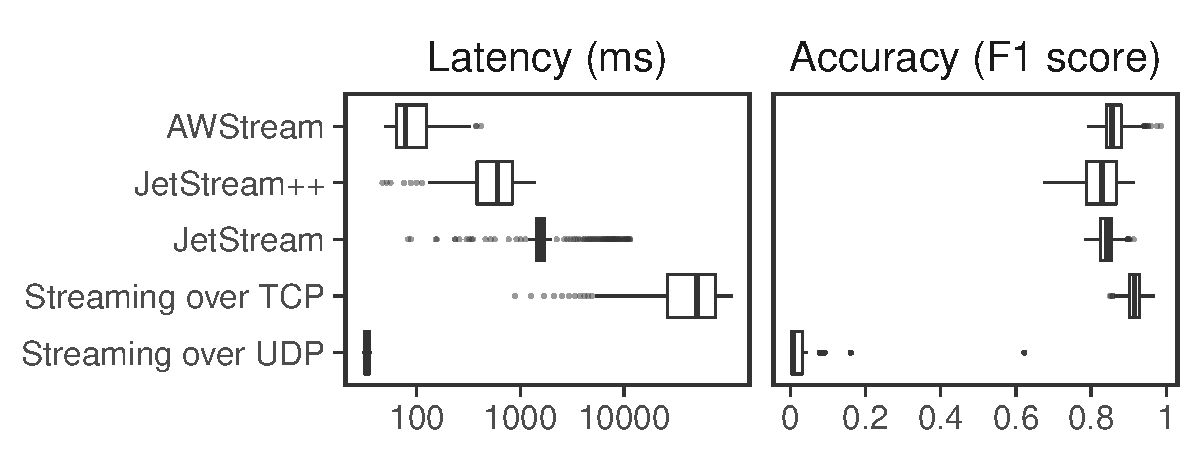
\includegraphics[width=\columnwidth]{figures/runtime_mot-boxplot.pdf}
    \caption{PD's performance summary of latency and accuracy during the traffic
      shaping (between t=200s and t=440s).}
\label{fig:pd-runtime-boxplot}
  \end{subfigure}
  \caption{PD runtime evaluation.}
  \label{fig:pd-runtime}
\end{figure}

\begin{figure}[t]
  \begin{subfigure}[t]{\columnwidth}
    \centering
    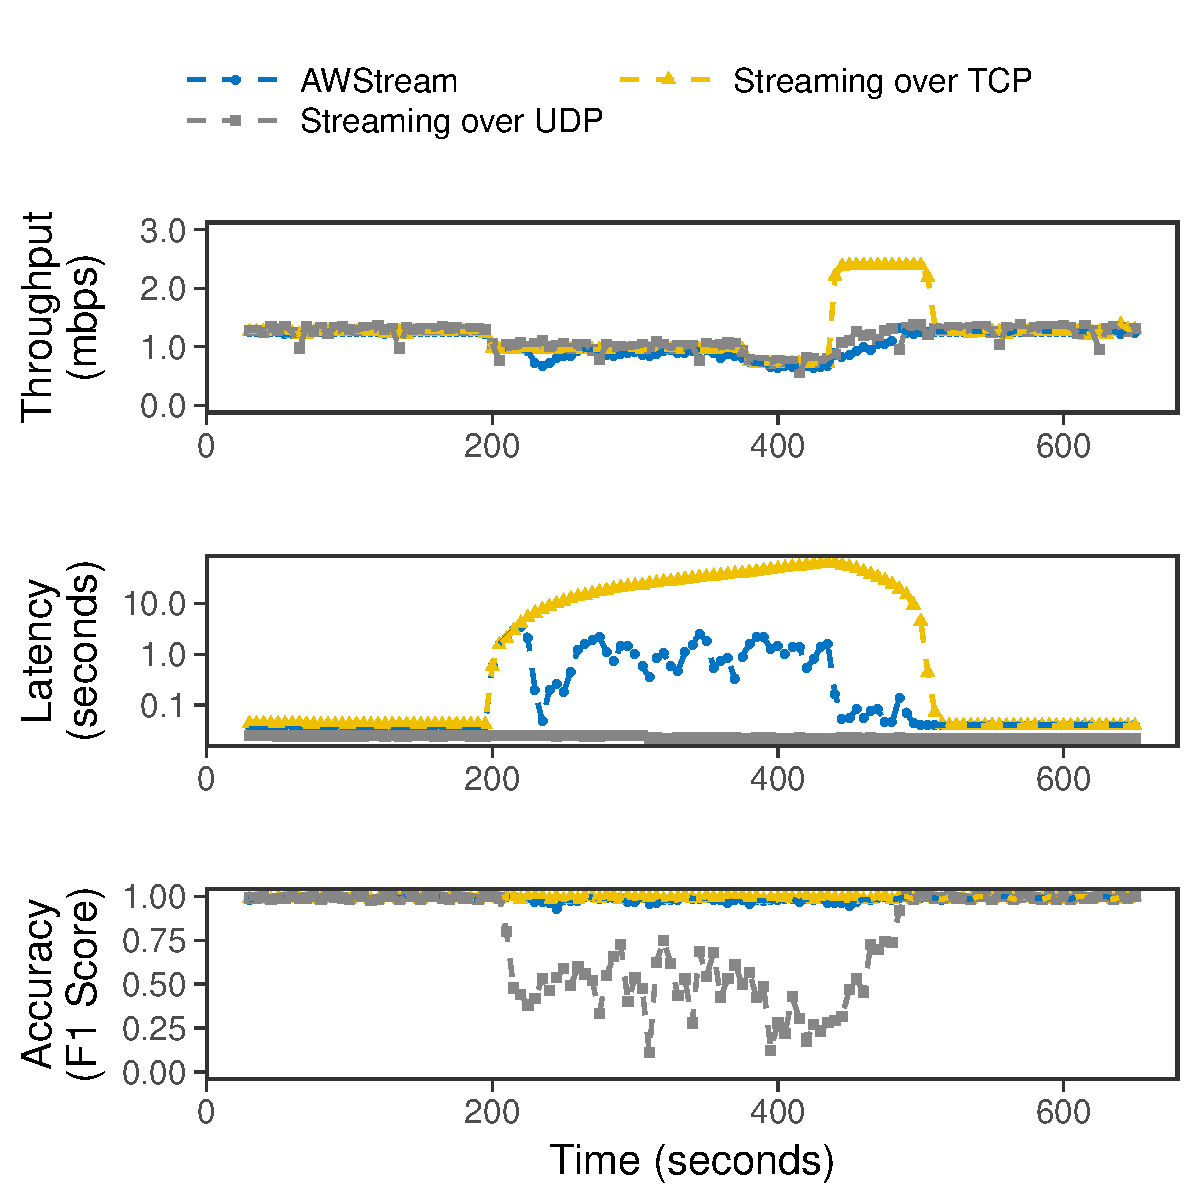
\includegraphics[width=\columnwidth]{figures/runtime_tk-timeseries.pdf}
    \caption{TK's runtime behavior with a time-series plot: throughput (top),
      showing the effect of bandwidth shaping; latency (middle) in log scale;
      and accuracy (bottom).}
    \label{fig:tk-runtime-timeseries}
  \end{subfigure}
  \vspace{1em}
  \\
  \begin{subfigure}[t]{\columnwidth}
    \centering
    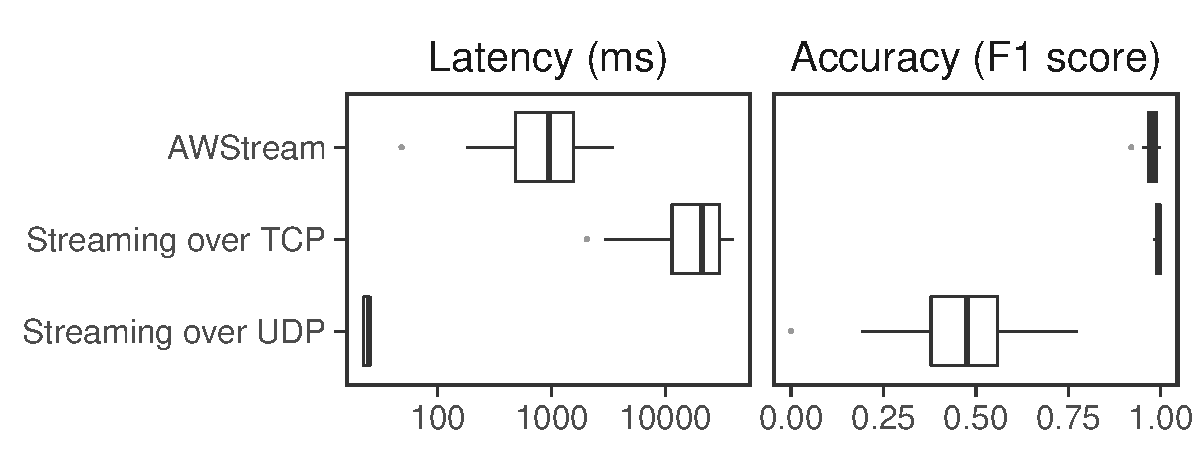
\includegraphics[width=\columnwidth]{figures/runtime_tk-boxplot.pdf}
    \caption{TK's performance summary of latency and accuracy during the traffic
      shaping (between t=200s and t=440s).}
    \label{fig:tk-runtime-boxplot}
  \end{subfigure}
  \caption{TK runtime evaluation.}
  \label{fig:tk-runtime}
\end{figure}

\paraf{Pedestrian Detection.} The setup for PD is the same with AR: three Amazon
EC2 as clients and one as server. The maximal configuration $c_{\max}$ is
1920x1080 resolution, \(10~\text{FPS}\) and a quantization of 20; it consumes
about 12 mbps. When running experiments, we use the same bandwidth shaping
schedule. Baselines are also the same: Streaming over TCP/UDP, JetStream, and
JetStream++.

\autoref{fig:pd-runtime} shows the runtime behavior of \sysname{} and all
baselines in time series (throughout the experiment) and box plot (between
t=200s and t=440s). The trend is quite similar to AR, so we omit a verbose
description.

\para{Top-K.} For TK, with our data is split into four groups, we use four
Amazon EC2 as clients and one as server. We also limit the maximal configuration
$c_{\max}$ as $N=9750$ for \texttt{head} and $T=0$ for \texttt{threshold}; it
consumes about 1.2 mbps. Because the overall bandwidth consumption is much
smaller than video analytics, we change the bandwidth parameter: during
t=200-380s, we limit the bandwidth to 750 kbps; during t=380-440s, the bandwidth
is 500 kbps. The background bandwidth limit is 2.5 mpbs.

We've only compared \sysname{} with two baselines: streaming over TCP and
streaming over UDP. For TCP baseline, we use AWStream but disable the
adaptation. For UDP baseline, we implemented a simple application
protocol---packetization and a custom header---so that the receiver can still
aggregate data in the presence of UDP packet loss.

\autoref{fig:tk-runtime} shows the evaluation results for Top-K
application. Streaming over TCP has the highest accuracy (\textasciitilde
99.7\%) but the worst latency (up to 40 seconds). Streaming over UDP has the low
latency but its accuracy is the worst (\textasciitilde 52\%). \sysname{}
achieves low latency (\textasciitilde 1.1 second) and high accuracy
(\textasciitilde 98\%) simultaneously. Notice that because TK's source generates
data every second after the window operation, one object in the queue leads to
one seconds latency. \sysname{} manages to avoid queues for most times.

% > summary(latency)
%       Time       Streaming over TCP Streaming over UDP    AWStream
%  Min.   :210.0   Min.   : 2036      Min.   :22.29      Min.   :  48.03
%  1st Qu.:251.2   1st Qu.:11438      1st Qu.:22.42      1st Qu.: 485.08
%  Median :292.5   Median :21014      Median :24.78      Median : 946.45
%  Mean   :292.5   Mean   :20590      Mean   :23.85      Mean   :1145.05
%  3rd Qu.:333.8   3rd Qu.:29662      3rd Qu.:24.87      3rd Qu.:1557.20
%  Max.   :375.0   Max.   :39434      Max.   :24.98      Max.   :3509.99
% > summary(accuracy)
%       Time       Streaming over TCP Streaming over UDP    AWStream
%  Min.   :210.0   Min.   :0.9808     Min.   :0.1097     Min.   :0.9284
%  1st Qu.:251.2   1st Qu.:0.9892     1st Qu.:0.4467     1st Qu.:0.9694
%  Median :292.5   Median :0.9967     Median :0.5329     Median :0.9800
%  Mean   :292.5   Mean   :0.9928     Mean   :0.5236     Mean   :0.9786
%  3rd Qu.:333.8   3rd Qu.:0.9977     3rd Qu.:0.6063     3rd Qu.:0.9883
%  Max.   :375.0   Max.   :0.9991     Max.   :0.7981     Max.   :0.9991

\section{JetStream++}
\label{appendix:jetstream++}

We modified the open source version of
JetStream\footnote{\url{https://github.com/princeton-sns/jetstream/}, commit
  bf0931b2d74d20fdf891669188feb84c96AF84} in order to use our profile to act as
manual policies. Because JetStream doesn't support simultaneous degradation in
multiple dimensions, we implemented a simple \texttt{VideoSource} operator that
understands how to change image resolutions, frame rate, and video encoding
quantization. At runtime, \texttt{VideoSource} queries congestion policy manager
and adjusts three dimensions simultaneously. This operator is then exposed to
Python-implemented control plane. We call this modified version JetStream++.

JetStream's code base is modular and extensible: the modifications include 53
lines for the header file, 171 lines for implementation, 75 lines for unit test,
and 49 lines of python as the application.

While extending JetStream with our profile is not challenging, JetStream++
performs degradation in a single operator and loses the composability. We could
modify JetStream to support degradation across multiple operators, but that
would require substantial changes to JetStream. Using JetStream++ with our
profile, the comparison is enough to illustrate the difference between
\sysname{} and JetStream's runtime.

Regarding Top-K application, although JetStream provides a Top-K implementation,
it is based on ``Three-Phase Uniform Threshold'' (TPUT) and not suitable for
low-latency Top-K monitoring, according to the original
paper~\cite{cao2004efficient}, \textit{``in our target environments the query is
  asked hourly or daily. The intervals between the queries are typically long
  enough that the top-k objects have changed completely.''} We did not implement
our Top-K degradation with JetStream because video analytics suffices the
purpose of comparison.

%% Patches: https://github.com/nebgnahz/jetstream-clone/pull/2/files

%%% Local Variables:
%%% mode: latex
%%% TeX-master: "awstream"
%%% End:
